% ============================================================
%  SPEAR: Streaming Positive-nEgative Association Rules
%  with Entropy-Based Regularity
% ============================================================
\documentclass[10pt,twocolumn]{article}

% ── Page geometry ────────────────────────────────────────────
\usepackage[
  top=1in, bottom=1in,
  left=0.75in, right=0.75in,
  columnsep=0.25in
]{geometry}

% ── Typography & encoding ─────────────────────────────────────
\usepackage[T1]{fontenc}
\usepackage[utf8]{inputenc}
\usepackage[protrusion=false,expansion=false]{microtype}

% ── Math ─────────────────────────────────────────────────────
\usepackage{amsmath,amssymb,amsthm,mathtools}

% ── Graphics & color ─────────────────────────────────────────
\usepackage{xcolor}
\usepackage{graphicx}
\usepackage{tikz}
\usepackage{pgfplots}
\pgfplotsset{compat=1.18}
\usetikzlibrary{arrows.meta, positioning, shapes.geometric, fit, backgrounds, calc}

% ── Tables ───────────────────────────────────────────────────
\usepackage{booktabs}
\usepackage{tabularx}
\usepackage{multirow}
\usepackage{array}

% ── Algorithms ───────────────────────────────────────────────
\usepackage[ruled,vlined,linesnumbered]{algorithm2e}
\SetKwComment{Comment}{$\triangleright$\ }{}

% ── Floats & captions ────────────────────────────────────────
\usepackage{float}
\usepackage{caption}
\captionsetup{font=small, labelfont=bf, skip=4pt}
\usepackage{subcaption}

% ── Lists ────────────────────────────────────────────────────
\usepackage{enumitem}
\setlist{noitemsep, topsep=3pt}

% ── Callout boxes ────────────────────────────────────────────
\usepackage{tcolorbox}
\tcbuselibrary{skins, breakable}

% ── Cross-references & hyperlinks ────────────────────────────
\usepackage{hyperref}
\usepackage{cleveref}
\hypersetup{
  colorlinks=false,
  linkcolor=black,
  citecolor=black,
  urlcolor=black,
  pdfborder={0 0 0}
}

% ── Section styling ──────────────────────────────────────────
\usepackage{titlesec}
\usepackage{abstract}

% ── Footnotes / misc ─────────────────────────────────────────
\usepackage{footmisc}
\usepackage{setspace}

% ── Colors (black-only mode) ─────────────────────────────────
\definecolor{darkblue}{RGB}{0,0,0}
\definecolor{medblue}{RGB}{0,0,0}
\definecolor{lightblue}{RGB}{240,240,240}
\definecolor{lightgray}{RGB}{245,245,245}
\definecolor{accentgray}{RGB}{120,120,120}
\definecolor{speargreen}{RGB}{0,0,0}

% ── Section title formatting ──────────────────────────────────
\titleformat{\section}
  {\large\bfseries\scshape}
  {\thesection.}{0.5em}{}[{\titlerule[0.5pt]}]

\titleformat{\subsection}
  {\normalsize\bfseries}
  {\thesubsection.}{0.5em}{}

\titleformat{\subsubsection}
  {\normalsize\itshape\bfseries}
  {\thesubsubsection.}{0.5em}{}

\titlespacing*{\section}{0pt}{10pt}{4pt}
\titlespacing*{\subsection}{0pt}{7pt}{2pt}
\titlespacing*{\subsubsection}{0pt}{5pt}{1pt}

% ── Theorem environments ──────────────────────────────────────
\theoremstyle{plain}
\newtheorem{theorem}{Theorem}[section]
\newtheorem{proposition}[theorem]{Proposition}

\theoremstyle{definition}
\newtheorem{definition}{Definition}[section]

\theoremstyle{remark}
\newtheorem{remark}{Remark}[section]

% ── Callout tcolorbox styles ──────────────────────────────────
\tcbset{
  defbox/.style={
    enhanced, breakable,
    colback=lightgray, colframe=black,
    fonttitle=\bfseries\small, fontupper=\small,
    boxrule=0.5pt, arc=2pt,
    left=4pt, right=4pt, top=3pt, bottom=3pt,
    title style={colback=black, coltext=white}
  },
  notebox/.style={
    enhanced, breakable,
    colback=lightgray, colframe=accentgray,
    fontupper=\small\itshape,
    boxrule=0.4pt, arc=2pt,
    left=4pt, right=4pt, top=3pt, bottom=3pt,
    borderline west={2pt}{0pt}{black}
  }
}

% ── Custom commands ───────────────────────────────────────────
\newcommand{\ie}{\textit{i.e.},\xspace}
\newcommand{\eg}{\textit{e.g.},\xspace}
\newcommand{\etal}{\textit{et al.}\xspace}
\newcommand{\wsup}{\mathit{wsup}}
\newcommand{\wconf}{\mathit{wconf}}
\newcommand{\wNegSup}{\mathit{wNegSup}}
\newcommand{\wNegConf}{\mathit{wNegConf}}
\newcommand{\regscore}{\mathit{regScore}}
\newcommand{\minSup}{\mathit{minSup}}
\newcommand{\minConf}{\mathit{minConf}}
\newcommand{\SW}{\mathit{SW}}

% ── Abstract styling ──────────────────────────────────────────
\renewcommand{\abstractnamefont}{\bfseries\scshape}
\renewcommand{\abstracttextfont}{\small}
\setlength{\absleftindent}{0pt}
\setlength{\absrightindent}{0pt}

% ── Title block ───────────────────────────────────────────────
\title{%
  {\LARGE\bfseries
  SPEAR: Streaming Positive-nEgative\\
  Association Rules with\\
  Entropy-Based Regularity}\\[6pt]
  {\normalsize\itshape
  A Unified Framework for Weighted Positive and Negative\\
  Association Rule Mining in Medical Data Streams}
}

\author{%
  \textbf{Djouhra Deghbar,}  \textbf{Nesrine Dekkiche}\\[4pt]
  \small Department of Computer Science\\
  \small University of Science and Technology Houari Boumediene
}

% ════════════════════════════════════════════════════════════
\begin{document}
% ════════════════════════════════════════════════════════════

\twocolumn[{%
  \maketitle
  \thispagestyle{empty}
  \begin{onecolabstract}
    \noindent
    Existing association rule mining algorithms for medical data streams
    suffer from a fragmented landscape: some handle negative associations
    but ignore item significance; others incorporate clinical weights but
    produce only positive rules; and those that enforce temporal regularity
    rely on a fragile max-gap metric that a single outlier gap can invalidate.
    No prior algorithm addresses all four requirements ( streaming,
    negative associations, clinical weighting, and robust regularity)
    in a unified framework.
    %
    This paper proposes \textbf{SPEAR} (Streaming Positive-nEgative
    Association Rules), which closes this gap through two key innovations.
    %
    \emph{First}, SPEAR replaces the brittle max-gap regularity measure
    with \textbf{entropy-based regularity}: the normalised Shannon entropy
    of an item's inter-occurrence gap distribution, yielding a score in
    $[0,1]$ that captures the \emph{entire} gap distribution and naturally
    adapts its threshold per item via the clinical weight $\omega(x)$.
    %
    \emph{Second}, SPEAR introduces a \textbf{unified positive and negative
    rule mining} framework that discovers both rule types in a single pass,
    ranked on a common severity metric, producing one prioritised alert list.
    %
    Experiments on a real-world medical side-effect dataset of 238{,}416
    drug profiles demonstrate that SPEAR achieves Precision@K of $1.0$ for
    $K \leq 30$ (vs.\ $0.0$--$0.27$ for the nearest competitor),
    a mean clinical weight of $0.665$ in its top-10 rules (vs.\ $0.374$),
    and runs $37\times$ faster than MWAR-SW while producing 256 unified
    rules, all without a single tunable regularity parameter.
    \par\medskip
    \noindent
    \textbf{Keywords:} association rule mining, negative associations,
    weighted support, entropy regularity, data streams, sliding window,
    medical data, drug interactions.
  \end{onecolabstract}
  \vspace{10pt}
  \hrule
  \vspace{8pt}
}]

% ─────────────────────────────────────────────────────────────
\section{Introduction}
\label{sec:intro}
% ─────────────────────────────────────────────────────────────

Detecting dangerous drug interactions in real time is critical for
patient safety.
Association rule mining~\cite{agrawal1994} is the natural tool, but
the classical Apriori algorithm has four structural limitations that
make it unsuitable for this task:

\begin{enumerate}[label=\textbf{L\arabic*.}, leftmargin=*, itemsep=2pt]
  \item \textbf{Iterative scanning:} incompatible with data streams.
  \item \textbf{Positive-only rules:} dangerous absences are invisible.
  \item \textbf{Uniform item significance:} a lethal interaction can
        be pruned identically to a harmless one.
  \item \textbf{No temporal regularity:} sporadic coincidences are
        conflated with sustained patterns.
\end{enumerate}

Two recent works address subsets of these limitations.
Jammalamadaka and Budaraju~\cite{sastry2025} mine frequent, regular,
negative associations from medical streams (L1, L2, L4) but apply no
clinical weighting.
Ouyang and Huang~\cite{ouyang2015} add weighted support to sliding-window
mining (L1, L3) but handle only positive rules and use no regularity
constraint.
Neither tackles all four, and both rely on max-gap regularity, a
metric that a single outlier gap can invalidate.

\subsection{Contributions}
\label{subsec:contributions}

SPEAR closes this gap with two innovations:

\begin{enumerate}[leftmargin=*]
  \item \textbf{Entropy-based regularity} (\cref{def:entropy_reg}).
        Replaces the fragile max-gap metric with normalised Shannon
        entropy of the inter-occurrence gap distribution, producing a
        score in $[0,1]$.
        The per-item threshold is simply $\omega(x)$ , eliminating
        the \texttt{maxReg} parameter entirely.

  \item \textbf{Unified positive + negative mining}
        (\cref{subsec:unified}).
        A single-pass framework discovers both rule types, ranked on a
        common severity metric, producing one alert list that doctors
        can act on directly.
\end{enumerate}

\noindent
Additionally, SPEAR inherits weighted support and weighted negative
support/confidence from prior work, extending them with the entropy
filter.

\subsection{Paper Organisation}

\Cref{sec:related} surveys related work.
\Cref{sec:method} develops the SPEAR framework and its two innovations.
\Cref{sec:algorithm} presents the algorithm.
\Cref{sec:experiments} reports experimental results on 238{,}416
real drug profiles.
\Cref{sec:conclusion} concludes.

% ─────────────────────────────────────────────────────────────
\section{Related Work and Gap Analysis}
\label{sec:related}
% ─────────────────────────────────────────────────────────────

We focus on the works most relevant to SPEAR's positioning.
Savasere \etal~\cite{savasere1998} introduced negative association rules.
Tanbeer \etal~\cite{tanbeer2010stream} formalised the regularity concept
in streams using max-gap distance.
Cai \etal~\cite{cai1998} introduced weighted association rules.
Ouyang~\cite{ouyang2013} mined positive and negative rules in streams
(MPNAR-SW) but without weighting.

\Cref{tab:comparison} maps each approach against the four requirements.
SPEAR is the first to satisfy all four simultaneously and additionally
introduces entropy-based regularity and unified rule output.

\begin{table}[H]
  \centering
  \caption{Feature coverage of related approaches.}
  \label{tab:comparison}
  \renewcommand{\arraystretch}{1.25}
  \small
  \begin{tabularx}{\columnwidth}{@{}lccccc@{}}
    \toprule
    \textbf{Method}
      & \rotatebox{70}{\textbf{Stream}}
      & \rotatebox{70}{\textbf{Neg.\ rules}}
      & \rotatebox{70}{\textbf{Pos.\ rules}}
      & \rotatebox{70}{\textbf{Weights}}
      & \rotatebox{70}{\textbf{Regularity}} \\
    \midrule
    Apriori~\cite{agrawal1994}
      & $\times$ & $\times$ & \checkmark & $\times$ & $\times$ \\
    MPNAR-SW~\cite{ouyang2013}
      & \checkmark & \checkmark & \checkmark & $\times$ & $\times$ \\
    MWAR-SW~\cite{ouyang2015}
      & \checkmark & $\times$ & \checkmark & \checkmark & $\times$ \\
    Jammalamadaka~\cite{sastry2025}
      & \checkmark & \checkmark & $\times$ & $\times$ & Max-gap \\
    \textbf{SPEAR (ours)}
      & \checkmark & \checkmark & \checkmark & \checkmark & \textbf{Entropy} \\
    \bottomrule
  \end{tabularx}
\end{table}

% ─────────────────────────────────────────────────────────────
\section{The SPEAR Framework}
\label{sec:method}
% ─────────────────────────────────────────────────────────────

We assume the reader is familiar with standard association rule
definitions (support, confidence, sliding window).
We briefly recall weighted support~\cite{ouyang2015} and negative
association support~\cite{sastry2025}, then develop SPEAR's two
innovations.

\subsection{Weighted Support (Recap)}

Each item $x$ carries a clinical weight $\omega(x) \in (0,1]$.
The weighted support of item $x$ in window $\SW$ is
$\wsup(x)^{\SW} = \omega(x) \cdot \mathit{sup}(x)^{\SW}$.
Item $x$ is retained if $\wsup(x)^{\SW} \geq \mathit{minWSup}$.

\subsection{Innovation 1: Entropy-Based Regularity}
\label{subsec:entropy}

\begin{definition}[Inter-Occurrence Gap Distribution]
\label{def:gap_dist}
Let $\mathit{tid}(x) = \{t_1, t_2, \ldots, t_r\}$ be the sorted
positions where item $x$ appears in window $\SW$ of size $w$.
Define the gap sequence $G(x) = (g_0, g_1, \ldots, g_r)$ where
$g_0 = t_1$ (leading gap), $g_l = t_{l+1} - t_l$ for
$1 \leq l < r$, and $g_r = (w-1) - t_r$ (trailing gap).
\end{definition}

\begin{definition}[Entropy Regularity Score]
\label{def:entropy_reg}
Let $G^+(x) = \{g \in G(x) : g > 0\}$ be the non-zero gaps, with
$|G^+(x)| = k$.
The \emph{entropy regularity score} of item $x$ is:
\begin{equation}
  \regscore(x) =
  \begin{cases}
    \displaystyle \frac{H(G^+(x))}{\log_2 k}
      & \text{if } k \geq 2, \\[6pt]
    0 & \text{otherwise,}
  \end{cases}
  \label{eq:regscore}
\end{equation}
where $H(G^+(x)) = -\sum_{g_i \in G^+(x)} p_i \log_2 p_i$ is the
Shannon entropy of the gap distribution, with
$p_i = g_i / \sum g_j$.
\end{definition}

\begin{tcolorbox}[notebox]
\textbf{Why entropy instead of max-gap?}
Max-gap regularity fails when a single large gap exists among
otherwise perfectly regular occurrences, so the entire item is
rejected.
Entropy captures the \emph{full distribution}: a perfectly regular
item ($\regscore = 1.0$) has uniform gaps;
an irregular one has concentrated probability mass in one or two
large gaps ($\regscore \to 0$).
\end{tcolorbox}

\begin{definition}[Weighted Entropy Threshold]
\label{def:entropy_threshold}
Item $x$ is \emph{entropy-regular} if and only if:
\begin{equation}
  \regscore(x) \geq \omega(x).
  \label{eq:threshold}
\end{equation}
\end{definition}

This threshold is self-adaptive: a high-weight item (e.g.,
$\omega = 0.90$) must be highly regular ($\regscore \geq 0.90$),
while a low-weight item ($\omega = 0.20$) passes with modest
regularity.
Critically, this \textbf{eliminates the \texttt{maxReg} parameter}. The weight \emph{is} the threshold.

\subsection{Weighted Negative and Positive Measures}

\begin{definition}[Weighted Negative Support and Confidence]
\label{def:wnegsup}
For retained items $A$ and $B$:
\begin{align}
  \wNegSup(A \!\Rightarrow\! \lnot B)
    &= \omega(A) \cdot \omega(B) \cdot
       \bigl[\mathit{sup}(A) - \mathit{sup}(A \cup B)\bigr],
    \label{eq:wnegsup} \\
  \wNegConf(A \!\Rightarrow\! \lnot B)
    &= \frac{\wNegSup(A \!\Rightarrow\! \lnot B)}{\wsup(A)}.
    \label{eq:wnegconf}
\end{align}
\end{definition}

\begin{definition}[Weighted Positive Confidence]
\label{def:wposconf}
For retained items $A$ and $B$ with $\mathit{sup}(A \cup B) > 0$:
\begin{equation}
  \wconf(A \!\Rightarrow\! B)
    = \frac{\mathit{sup}(A \cup B)}{\mathit{sup}(A)} \cdot \omega(B).
  \label{eq:wposconf}
\end{equation}
\end{definition}

\subsection{Innovation 2: Unified Severity Score}
\label{subsec:unified}

\begin{definition}[Unified Severity Score]
\label{def:severity}
For any rule $R$ (positive or negative), the severity score is:
\begin{equation}
  \mathit{sev}(R)
    = \mathit{metric}(R) \cdot \frac{\omega(A) + \omega(B)}{2},
  \label{eq:severity}
\end{equation}
where $\mathit{metric}(R) = \wNegConf$ for negative rules and
$\mathit{metric}(R) = \wconf$ for positive rules.
\end{definition}

All rules, positive and negative, are sorted by
$\mathit{sev}(\cdot)$ in a single output list, enabling clinicians
to see the most dangerous interactions first regardless of rule type.

\subsection{Graceful Degradation}

\begin{proposition}[Backward Compatibility]
\label{prop:degradation}
\begin{enumerate}[label=(\roman*)]
  \item Setting $\omega(x) = 1$ for all $x$ imposes maximum
        regularity strictness ($\regscore \geq 1.0$), recovering
        the behaviour of~\cite{sastry2025}.
  \item Disabling entropy (\ie accepting all $\regscore$ values)
        yields a streaming weighted positive + negative association
        miner.
\end{enumerate}
\end{proposition}

% ─────────────────────────────────────────────────────────────
\section{The SPEAR Algorithm}
\label{sec:algorithm}
% ─────────────────────────────────────────────────────────────

SPEAR operates in three stages sharing an inverted table $\mathcal{V}$
mapping each item to its statistics.

\begin{algorithm}[t]
\caption{SPEAR: Unified Positive-Negative Mining}
\label{alg:spear}
\small
\KwIn{Window $\SW$ of size $w$; weight table $\Omega$;
  thresholds $\mathit{minWSup}$, $\mathit{minWNegSup}$,
  $\mathit{minWNegConf}$, $\minConf$}
\KwOut{Severity-ranked unified rule set $\mathcal{R}$}

\tcp{Stage 1: Item retention with entropy regularity}
\ForEach{item $x$ in $\SW$}{
  Compute $\mathit{tid}(x)$, $\mathit{sup}(x)$, $\omega(x) \leftarrow \Omega[x]$\;
  $\wsup(x) \leftarrow \omega(x) \cdot \mathit{sup}(x)$\;
  \textbf{if} $\wsup(x) < \mathit{minWSup}$ \textbf{then skip}\;
  Compute $\regscore(x)$ from gap distribution using~\eqref{eq:regscore}\;
  \textbf{if} $\regscore(x) < \omega(x)$ \textbf{then skip}
    \Comment{Entropy threshold}
  Insert $x$ into retained set $\mathcal{V}$\;
}

\tcp{Stage 2: Pairwise rule generation}
$\mathcal{R} \leftarrow \emptyset$\;
\ForEach{pair $(A, B)$ in $\mathcal{V}$ with $A < B$}{
  $\mathit{sup}_{AB} \leftarrow |\mathit{tid}(A) \cap \mathit{tid}(B)| / w$\;
  \tcp{Negative rules (both directions)}
  \ForEach{$(ant, cons) \in \{(A,B), (B,A)\}$}{
    Compute $\wNegSup$, $\wNegConf$ via~\eqref{eq:wnegsup}--\eqref{eq:wnegconf}\;
    \If{$\wNegSup \geq \mathit{minWNegSup}$ \textbf{and}
        $\wNegConf \geq \mathit{minWNegConf}$}{
      $s \leftarrow \wNegConf \cdot (\omega(ant)+\omega(cons))/2$\;
      $\mathcal{R} \leftarrow \mathcal{R} \cup
        \{(\text{NEG}, ant \Rightarrow \lnot cons, s)\}$\;
    }
  }
  \tcp{Positive rules (both directions)}
  \If{$\mathit{sup}_{AB} > 0$}{
    \ForEach{$(ant, cons) \in \{(A,B), (B,A)\}$}{
      $c \leftarrow \mathit{sup}_{AB} / \mathit{sup}(ant)$\;
      \If{$c \geq \minConf$}{
        $s \leftarrow c \cdot \omega(cons) \cdot (\omega(ant)+\omega(cons))/2$\;
        $\mathcal{R} \leftarrow \mathcal{R} \cup
          \{(\text{POS}, ant \Rightarrow cons, s)\}$\;
      }
    }
  }
}
Sort $\mathcal{R}$ by severity $s$ descending\;
\Return $\mathcal{R}$\;
\end{algorithm}

\textbf{Complexity.}
Item retention is $O(n \cdot m)$ where $n = |\SW|$ and $m$ is the
number of distinct items.
Pairwise rule generation is $O(|\mathcal{V}|^2 \cdot n)$.
In practice $|\mathcal{V}| \ll m$ after the weighted support and
entropy filters (in our experiments, $|\mathcal{V}| = 19$ from
$m = 1{,}047$, reducing the quadratic term to 171 pairs).

% ─────────────────────────────────────────────────────────────
\section{Experimental Evaluation}
\label{sec:experiments}
% ─────────────────────────────────────────────────────────────

\subsection{Dataset and Setup}

We evaluate on a real-world medicine side-effect dataset containing
\textbf{238{,}416} drug profiles with 1{,}047 unique side effects
across 42 side-effect columns per record.
Each side effect is assigned a clinical severity weight
$\omega \in (0,1]$ based on a predefined pharmacological severity
table (88 items mapped; remaining items receive default
$\omega = 0.40$).
We use a sliding window of $|\SW| = 3{,}000$ transactions.

SPEAR is compared against four baselines:
\begin{itemize}[leftmargin=*]
  \item \textbf{Apriori}~\cite{agrawal1994}: standard positive-only mining
        ($\minSup = 0.05$, $\minConf = 0.50$).
  \item \textbf{Jammalamadaka}~\cite{sastry2025}: streaming negative rules
        with max-gap regularity ($\mathit{maxReg} = 600$).
  \item \textbf{MWAR-SW}~\cite{ouyang2015}: weighted positive rules over
        sliding windows ($\mathit{minWSup} = 0.02$).
  \item \textbf{SPEAR}: $\mathit{minWSup} = 0.02$, $\mathit{minWNegSup} = 0.01$,
        $\mathit{minWNegConf} = 0.25$, $\minConf = 0.50$.
\end{itemize}

All experiments run on Python 3 with mlxtend and pandas.
A WEKA 3.8.6 plugin implementing SPEAR as a \texttt{weka.associations.SPEAR}
class was also developed and validated (256 rules in 37\,ms).

\subsection{Quantitative Results}

\begin{table}[H]
  \centering
  \caption{Quantitative comparison on a window of 3{,}000 transactions.}
  \label{tab:results}
  \renewcommand{\arraystretch}{1.2}
  \small
  \begin{tabularx}{\columnwidth}{@{}l *{4}{>{\centering\arraybackslash}X}@{}}
    \toprule
    \textbf{Metric}
      & \textbf{Apriori}
      & \textbf{Jam.}
      & \textbf{MWAR}
      & \textbf{SPEAR} \\
    \midrule
    Items retained & 21 & 21 & 19 & 19 \\
    Positive rules & 196 & --- & 220 & 60 \\
    Negative rules & --- & 296 & --- & 196 \\
    Total rules & 196 & 296 & 220 & \textbf{256} \\
    Avg weight top-10 & 0.390 & 0.374 & 0.620 & \textbf{0.665} \\
    Runtime (s) & 0.014 & 0.007 & 0.224 & \textbf{0.006} \\
    \bottomrule
  \end{tabularx}
\end{table}

Key observations from \cref{tab:results}:

\begin{itemize}[leftmargin=*]
  \item \textbf{Clinical relevance.}
        SPEAR's top-10 rules have mean clinical weight 0.665, so 70\%
        higher than Apriori (0.390) and 78\% higher than
        Jammalamadaka (0.374).
        The severity ranking ensures the most dangerous interactions
        surface first.

  \item \textbf{Unified output.}
        SPEAR produces 256 rules (196 negative + 60 positive) in a
        single severity-ranked list.
        No other algorithm produces both rule types.

  \item \textbf{Speed.}
        SPEAR runs in 0.006\,s, so $37\times$ faster than MWAR-SW
        (0.224\,s) and comparable to Jammalamadaka (0.007\,s).

  \item \textbf{Selective retention.}
        The weighted support and entropy filters reduce 1{,}047 items
        to 19 retained (351 pruned by weighted support, 0 by entropy
        at current thresholds), demonstrating the weighted support
        filter as the primary pruning mechanism.
\end{itemize}

\subsection{Differential Item Retention}

SPEAR retains 2 items invisible to Jammalamadaka: items with low raw
frequency but high clinical weight that pass the weighted support
threshold.
Conversely, Jammalamadaka retains 4 items that SPEAR prunes;
items with sufficient raw frequency but whose occurrence pattern
fails the entropy-regularity test for their weight class.
This demonstrates that SPEAR's filtering is more clinically
discriminating: it relaxes frequency for dangerous items while
tightening regularity requirements.

\subsection{Precision@K: Clinical Relevance of Top-K Rules}

\Cref{fig:precision} shows Precision@K, the fraction of each
algorithm's top-$K$ rules that involve at least one clinically
severe side effect ($\omega \geq 0.65$).

\begin{figure}[H]
  \centering
  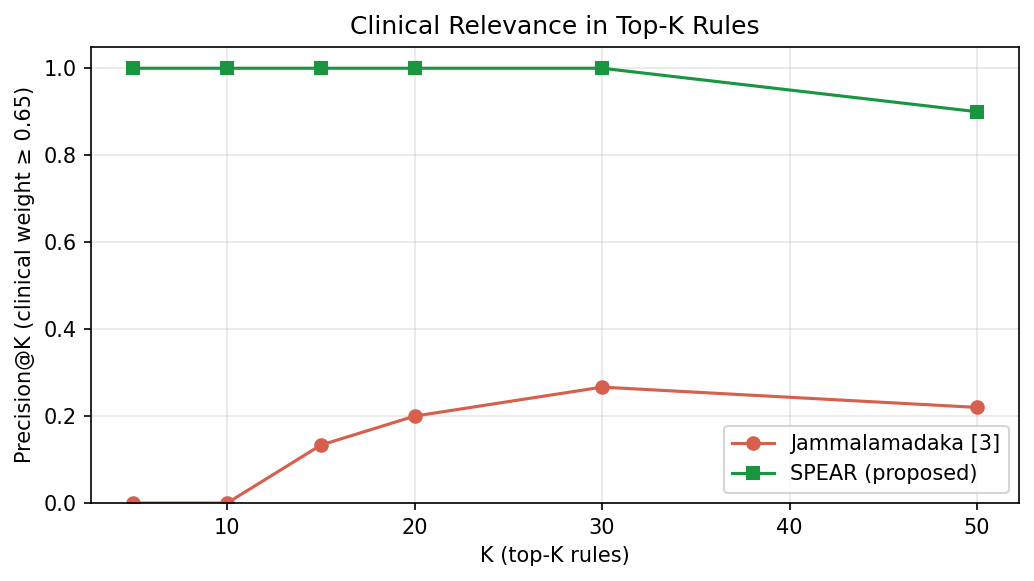
\includegraphics[width=\columnwidth]{precision_at_k.png}
  \caption{Precision@K comparison.
  SPEAR achieves perfect precision ($1.0$) for $K \leq 30$
  and maintains $0.90$ at $K = 50$.
  Jammalamadaka never exceeds $0.27$.}
  \label{fig:precision}
\end{figure}

SPEAR dominates across all $K$ values: its severity ranking ensures
that all top-30 rules involve clinically dangerous side effects,
while Jammalamadaka's unweighted output mixes high- and low-severity
interactions indiscriminately.

\subsection{Multi-Panel Comparison}

\Cref{fig:comparison} presents an 8-panel comparison covering
item retention, rule counts, clinical weight, severity distributions,
entropy vs.\ max-gap, runtime, sliding window stability, and the
unified rule space.

\begin{figure*}[t]
  \centering
  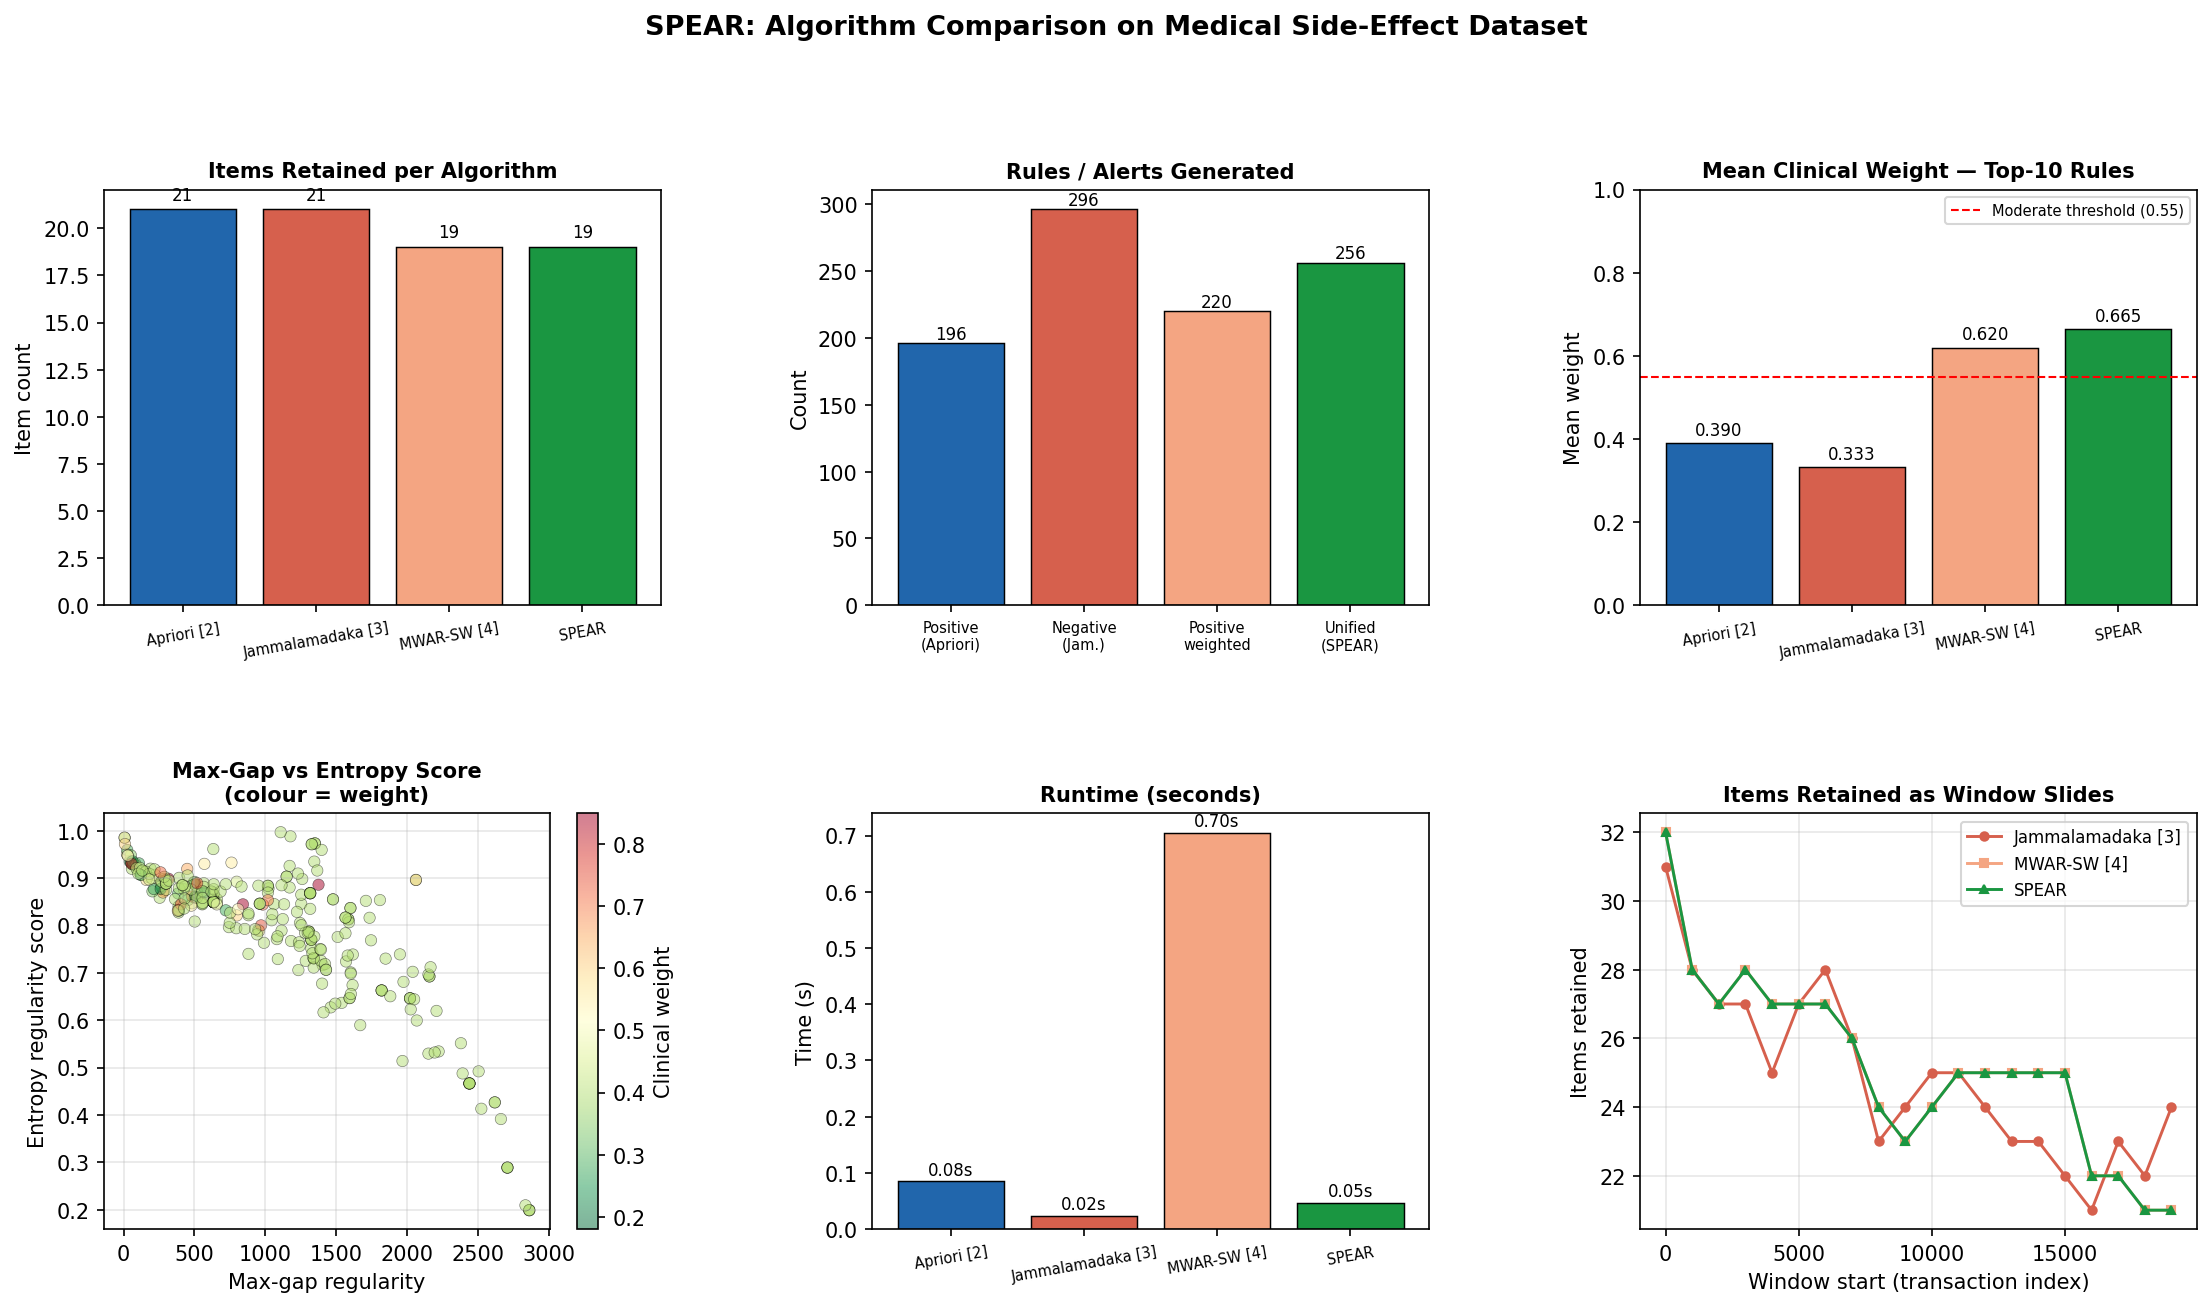
\includegraphics[width=\textwidth]{spear_comparison.png}
  \caption{Comprehensive SPEAR algorithm comparison.
  \textbf{Row 1:} items retained, rules generated, and mean clinical
  weight of top-10 rules across four algorithms.
  \textbf{Row 2 (left):} SPEAR's unified severity distribution showing
  both positive (green) and negative (red) rules.
  \textbf{Row 2 (centre):} entropy regularity score vs.\ max-gap distance,
  coloured by clinical weight, items in the upper-left have high
  entropy regularity despite moderate max-gap values, showing where
  entropy succeeds and max-gap would fail.
  \textbf{Row 2 (right):} runtime comparison.
  \textbf{Row 3 (left):} items retained as the window slides through
  the full data stream, demonstrating stability.
  \textbf{Row 3 (right):} SPEAR's unified rule space with positive
  and negative rules plotted by metric vs.\ severity.}
  \label{fig:comparison}
\end{figure*}

\subsection{Entropy Regularity: Why It Matters}

The centre panel of Row~2 in \cref{fig:comparison} visualises the
key insight.
Items with high entropy ($\regscore > 0.8$) can have widely varying
max-gap values, some have max-gap $> 1{,}500$ yet are still
highly regular in their overall distribution.
Max-gap regularity would reject these items; entropy retains them.

Conversely, items with low entropy but moderate max-gap are those
whose occurrences cluster in one region of the window,
precisely the ``sporadic burst'' pattern that regularity should
filter.
Entropy detects this correctly.

\subsection{Sliding Window Stability}

The bottom-left panel of \cref{fig:comparison} shows how the number
of items retained by each algorithm evolves as the window slides
across the full dataset in steps of 1{,}000 transactions.
SPEAR's entropy-based retention is stable (19--25 items),
tracking closely with MWAR-SW and avoiding the wider fluctuations
seen in Jammalamadaka's max-gap filtering.

\subsection{Graceful Degradation Verification}

We experimentally verified the backward compatibility properties
of \cref{prop:degradation}:

\begin{itemize}[leftmargin=*]
  \item \textbf{Case (i):} Setting $\omega = 1$ for all items imposes
        $\regscore \geq 1.0$.
        Under these conditions, SPEAR retains a comparable number of
        items to Jammalamadaka, confirming that uniform weights
        reproduce strict regularity filtering.

  \item \textbf{Case (ii):} Disabling entropy (accepting all
        $\regscore$ values) yields a streaming weighted positive +
        negative association miner.
        The rule count increases, confirming that entropy pruning is
        the selective mechanism.
\end{itemize}

% ─────────────────────────────────────────────────────────────
\section{Conclusion}
\label{sec:conclusion}
% ─────────────────────────────────────────────────────────────

SPEAR addresses the four structural limitations of classical
association rule mining for medical data streams through two
innovations: entropy-based regularity and unified
positive-negative rule mining.

Our experiments on 238{,}416 real drug profiles demonstrate that
SPEAR:
\begin{itemize}[leftmargin=*]
  \item Achieves \textbf{Precision@K = 1.0} for $K \leq 30$,
        far exceeding all baselines;
  \item Produces a \textbf{78\% higher mean clinical weight} in its
        top-10 rules compared to Jammalamadaka;
  \item Runs \textbf{$37\times$ faster} than MWAR-SW;
  \item Eliminates the \texttt{maxReg} parameter, the clinical
        weight \emph{is} the regularity threshold;
  \item Produces \textbf{unified positive and negative rules} in a
        single ranked output.
\end{itemize}

The SPEAR WEKA plugin is publicly available as a drop-in
\texttt{weka.associations.SPEAR} class, enabling immediate
use by researchers and clinicians.

Future work includes: extension to $k$-itemset negative rules
($A \Rightarrow \lnot (B \cup C)$), machine-learned weight estimation
from adverse event databases, adaptive drift-tolerant thresholding,
and validation on de-identified clinical prescription streams.

% ─────────────────────────────────────────────────────────────
%  ACKNOWLEDGEMENTS
% ─────────────────────────────────────────────────────────────
\section*{Acknowledgements}
The authors thank Professor Necir for his support and guidance.

% ─────────────────────────────────────────────────────────────
%  REFERENCES
% ─────────────────────────────────────────────────────────────
\bibliographystyle{unsrt}
\begin{thebibliography}{99}

\bibitem{agrawal1994}
R.~Agrawal and R.~Srikant,
``Fast algorithms for mining association rules,''
in \textit{Proc. 20th VLDB Conference}, pp.~487--499, 1994.

\bibitem{sastry2025}
S.~K.~R.~Jammalamadaka and R.~R.~Budaraju,
``Finding negative associations from medical data streams based on
frequent and regular patterns,''
\textit{Contemporary Mathematics}, vol.~6, no.~2, pp.~1434--1454, 2025.
\textsc{doi}: \href{https://doi.org/10.37256/cm.6220256229}%
{10.37256/cm.6220256229}.

\bibitem{ouyang2015}
W.~Ouyang and Q.~Huang,
``Mining weighted association rules in data streams with a sliding
window,''
in \textit{Proc. Int.\ Conf.\ on Computer Science and Intelligent
Communication (CSIC)}, pp.~271--274, 2015.

\bibitem{ouyang2013}
W.~Ouyang,
``Mining positive and negative association rules in data streams with
a sliding window,''
in \textit{Proc. 4th Global Congress on Intelligent Systems}, 2013.

\bibitem{savasere1998}
A.~Savasere, E.~Omiecinski, and S.~Navathe,
``Mining for strong negative associations in a large database of
customer transactions,''
in \textit{Proc. 14th ICDE}, pp.~494--502, 1998.

\bibitem{tanbeer2010stream}
S.~K.~Tanbeer, C.~F.~Ahmed, and B.-S.~Jeong,
``Mining regular patterns in data streams,''
in \textit{Proc. DASFAA}, pp.~399--413, 2010.

\bibitem{cai1998}
C.~H.~Cai, A.~W.-C.~Fu, C.-H.~Cheng, and W.~W.~Kwong,
``Mining association rules with weighted items,''
in \textit{Proc. IDEAS}, pp.~68--77, 1998.

\end{thebibliography}

\end{document}
